\section{Temporal Models}
\label{sec:temporalModelsResults}

This chapter describes the results of the most essential experiments with sequential models.
These include the last ten models from \autoref{tab:temporalExperimetparams}.
For a fair comparison, all those models are trained for 100 epochs, the same window length of 10, and on the same version of the temporal dataset.
Additionally, the data augmentation strategy remains consistent.

Results are captured from inferring models on a video that includes scenes from the test set of the temporal dataset.
The auto-cropping mechanism is also utilized to be as close to a practical application as possible.
Furthermore, inference starts over 500 frames before the annotated sequence to give crop coordinates time to converge to their optimal positions.
This process results in \ac{IoU}s for each frame.
Consequently, \ac{IoU} trends for each model are plotted in \autoref{fig:IoUTrends}.
The evaluation includes all models using the original and the adapted auto-crop to ensure thoroughness.

Since sequences also include frames in which the train is located before the switch, these frames are excluded.
Only the most problematic frames for single-frame-based models in which the train is directly over the switch and the switchblades are not visible are considered.
The real switch-\ac{IoU}s and their corresponding frames included in this evaluation are marked with a green area in \autoref{fig:IoUTrends}.
The \ac{IoU}-trends show either a drop in accuracy or a rapid fluctuation.
After those irregularities, models usually recover and show stable predictions again.
These trends are expected from the behavior of uncertain models.
Either the model chooses the wrong track at a switch, which results in a drop, or the prediction varies between the right and wrong track, which leads to a fluctuation like in \autoref{fig:IoUTrends_switch_3}.
However, even though temporal models show similar behavior, it is visible that at least one model acts more robustly in sequences 2, 3 and 4.
Either the model is more stable overall, or the drop in accuracy is time-delayed.

\autoref{fig:IoUTrends} shows all trends of \ac{IoU}s for the 23 different methods listed in \autoref{tab:temporalModelsResults}.
However, only 6 of them are highlighted in colors.
The original model with the original auto-crop mechanism of \cite{tepNet2024} is in blue.
Then, the adapted single-frame-based model with the adapted and the original auto-crop (ogA) is shown in yellow and green.
Also included are the models CNN\_FC\_LSTM (ogA) and CNN\_FC\_FCOUT\_V1 in purple and cyan, which are the models with the highest average \ac{IoU} across all switches and switches 3 and 4, respectively.
Furthermore, the red trend is the best-performing temporal model for each corresponding scene.
In the first two graphs of \autoref{fig:IoUTrends}, CNN\_FC\_LSTM (ogA) is also the best-performing temporal model for these scenes.
Therefore, only the red one is visible.
\autoref{tab:temporalModelsResultsIoUsSummary} summarizes the \ac{IoU}s with the averages for the highlighted models across the switch scenarios.

% relevanten Switches größer
%\begin{figure}[H]
%    \centering
%    % Erste Reihe
%    \begin{subfigure}[b]{0.49\textwidth}
%        \centering
%        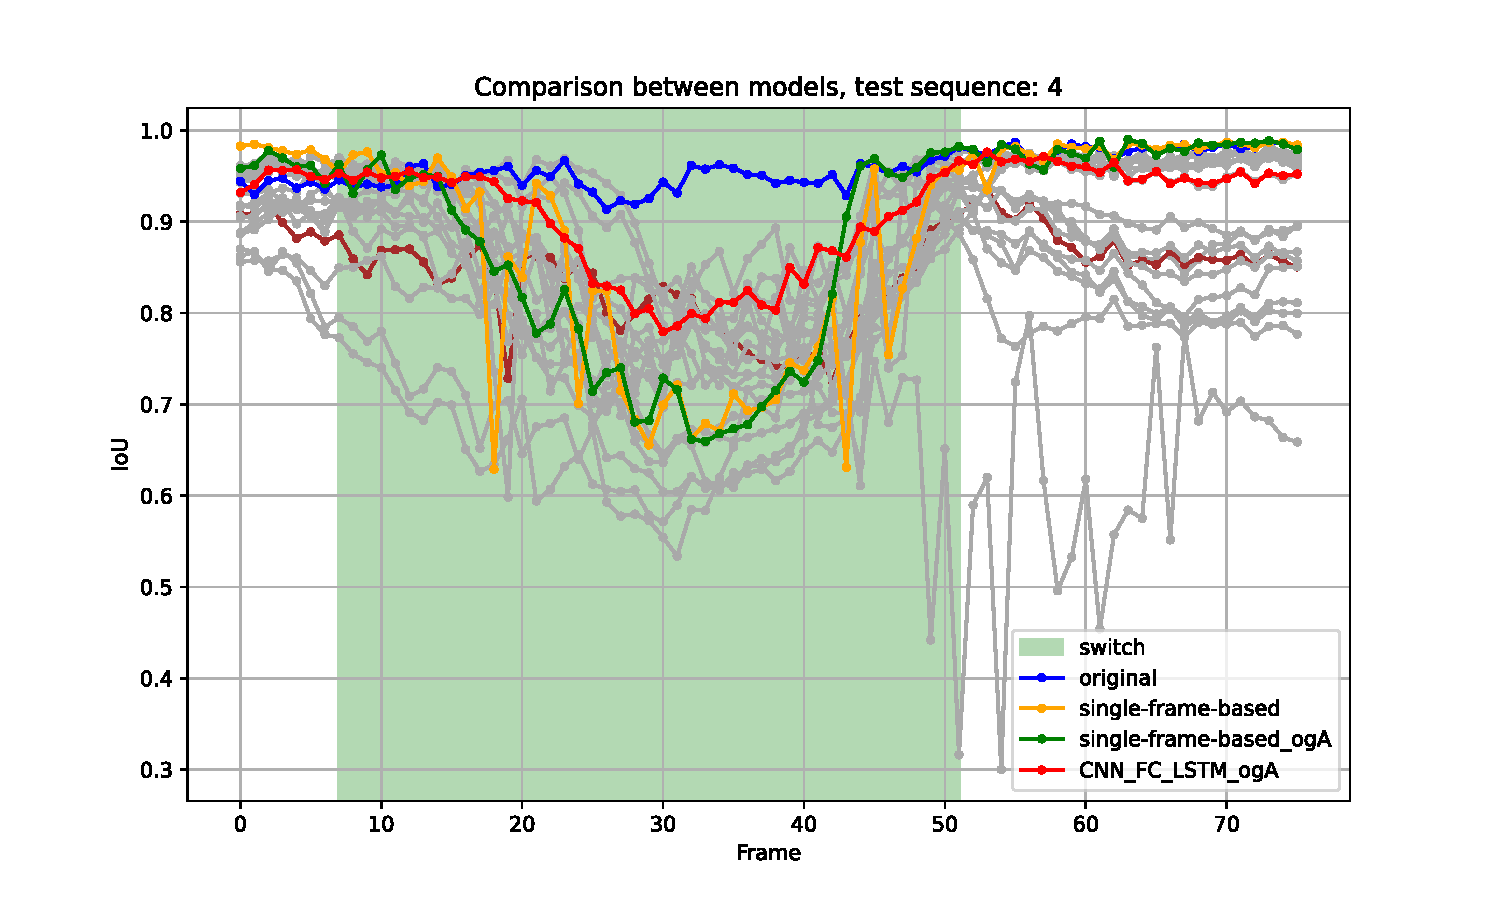
\includegraphics[width=\textwidth]{PICs/experiments/temporalModels/plot_ious_sequence_4.pdf}
%        \caption{Switch 1}
%        \label{fig:IoUTrends_switch_4}
%    \end{subfigure}
%    %\hfill
%    \begin{subfigure}[b]{0.49\textwidth}
%        \centering
%        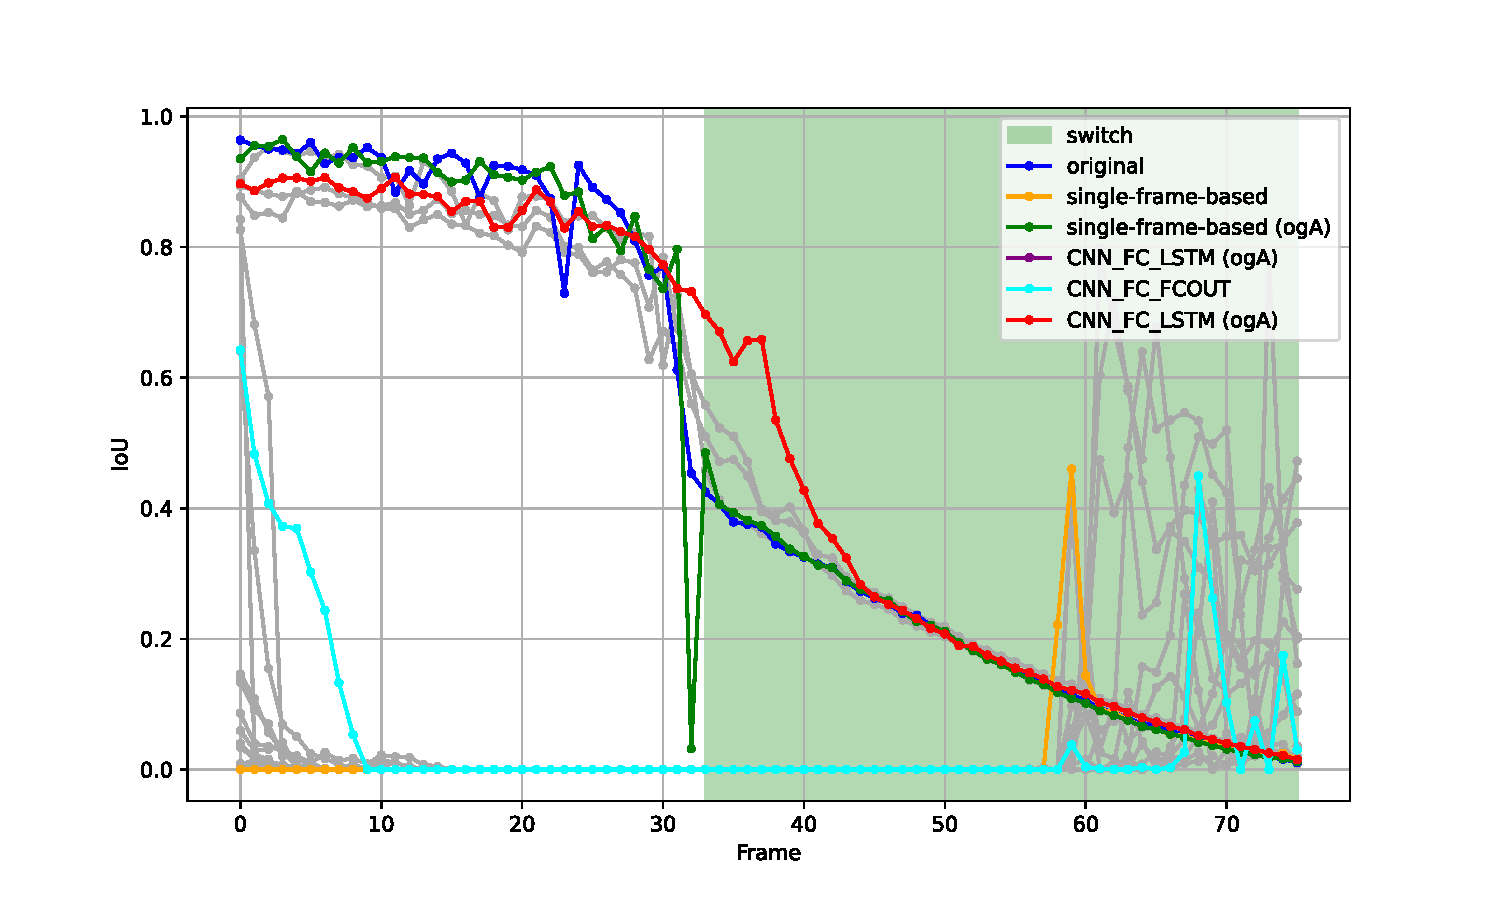
\includegraphics[width=\textwidth]{PICs/experiments/temporalModels/plot_ious_sequence_2.pdf}
%        \caption{Switch 2}
%        \label{fig:IoUTrends_switch_2}
%    \end{subfigure}
%
%    \vspace{1em} % Vertikaler Abstand zwischen den Reihen
%
%    % Zweite Reihe
%    \begin{subfigure}[b]{1\textwidth}
%        \centering
%        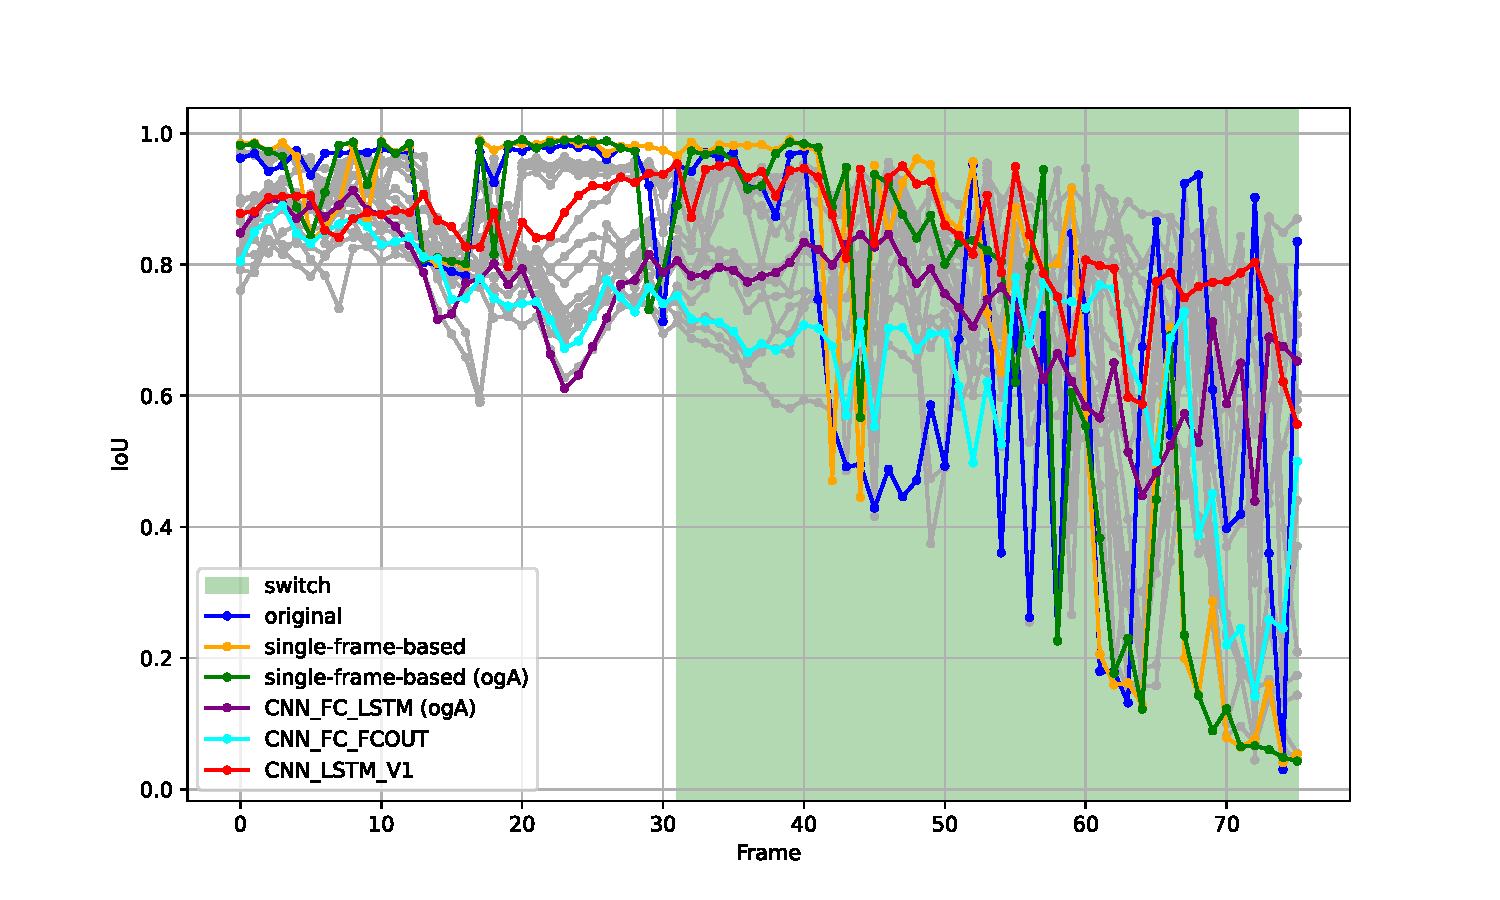
\includegraphics[width=0.8\textwidth]{PICs/experiments/temporalModels/plot_ious_sequence_3.pdf}
%        \caption{Switch 3}
%        \label{fig:IoUTrends_switch_3}
%    \end{subfigure}
%    %\hfill
%    \begin{subfigure}[b]{1\textwidth}
%        \centering
%        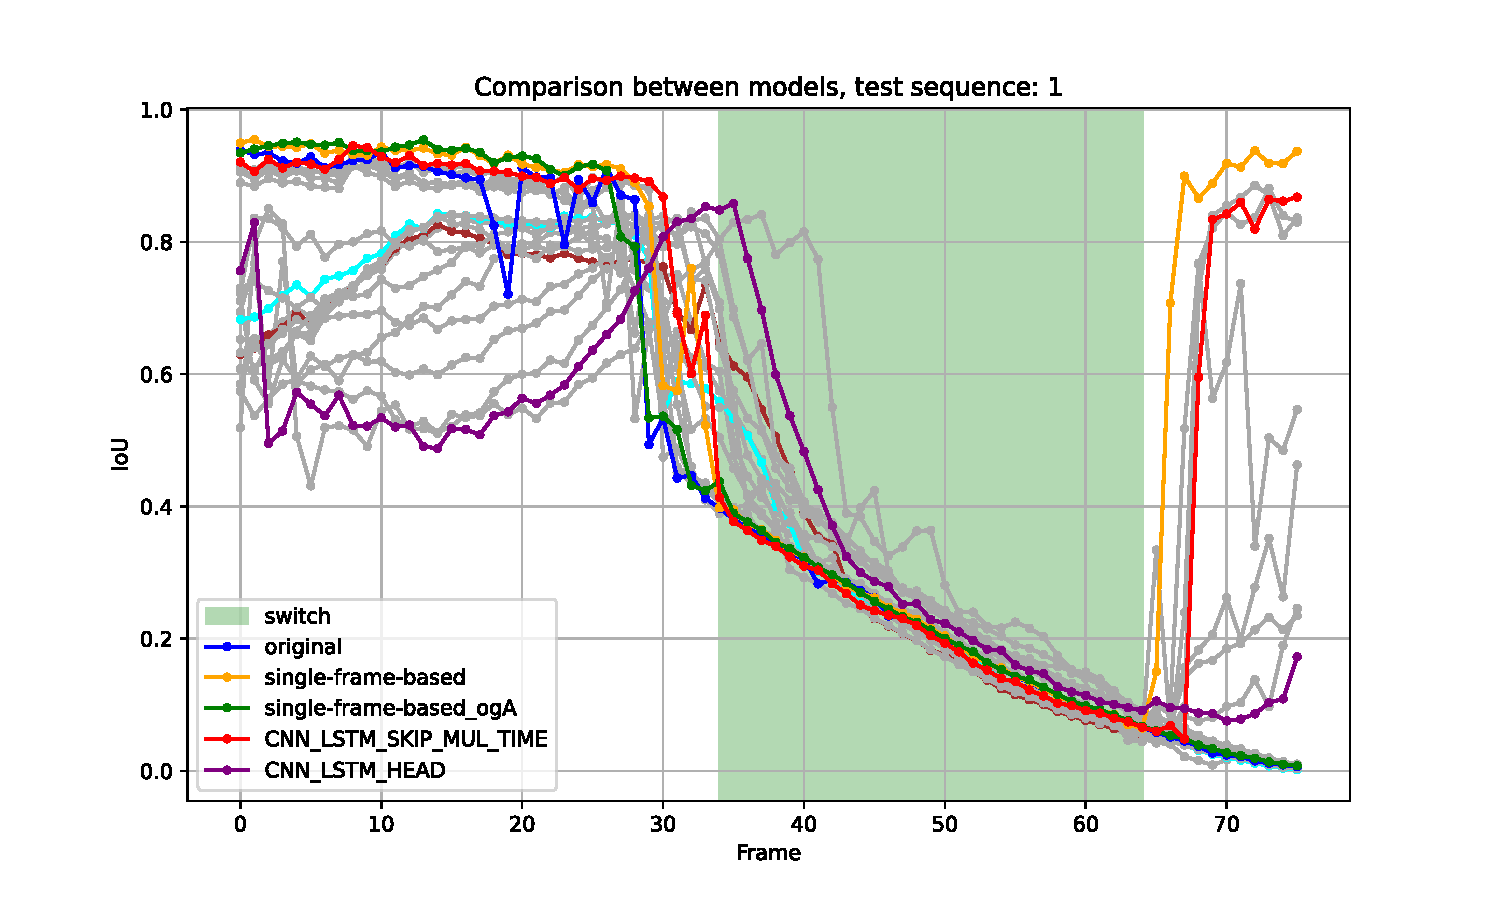
\includegraphics[width=0.8\textwidth]{PICs/experiments/temporalModels/plot_ious_sequence_1.pdf}
%        \caption{Switch 4}
%        \label{fig:IoUTrends_switch_1}
%    \end{subfigure}
%
%    \caption{\ac{IoU}-Trends of all models on the temporal test dataset with four sequences. Red is the best-performing temporal model for the corresponding sequence.}
%    \label{fig:IoUTrends}
%\end{figure}

% 2x2 raster
\begin{figure}[H]
    \centering
    \begin{subfigure}[b]{0.49\textwidth}
        \centering
        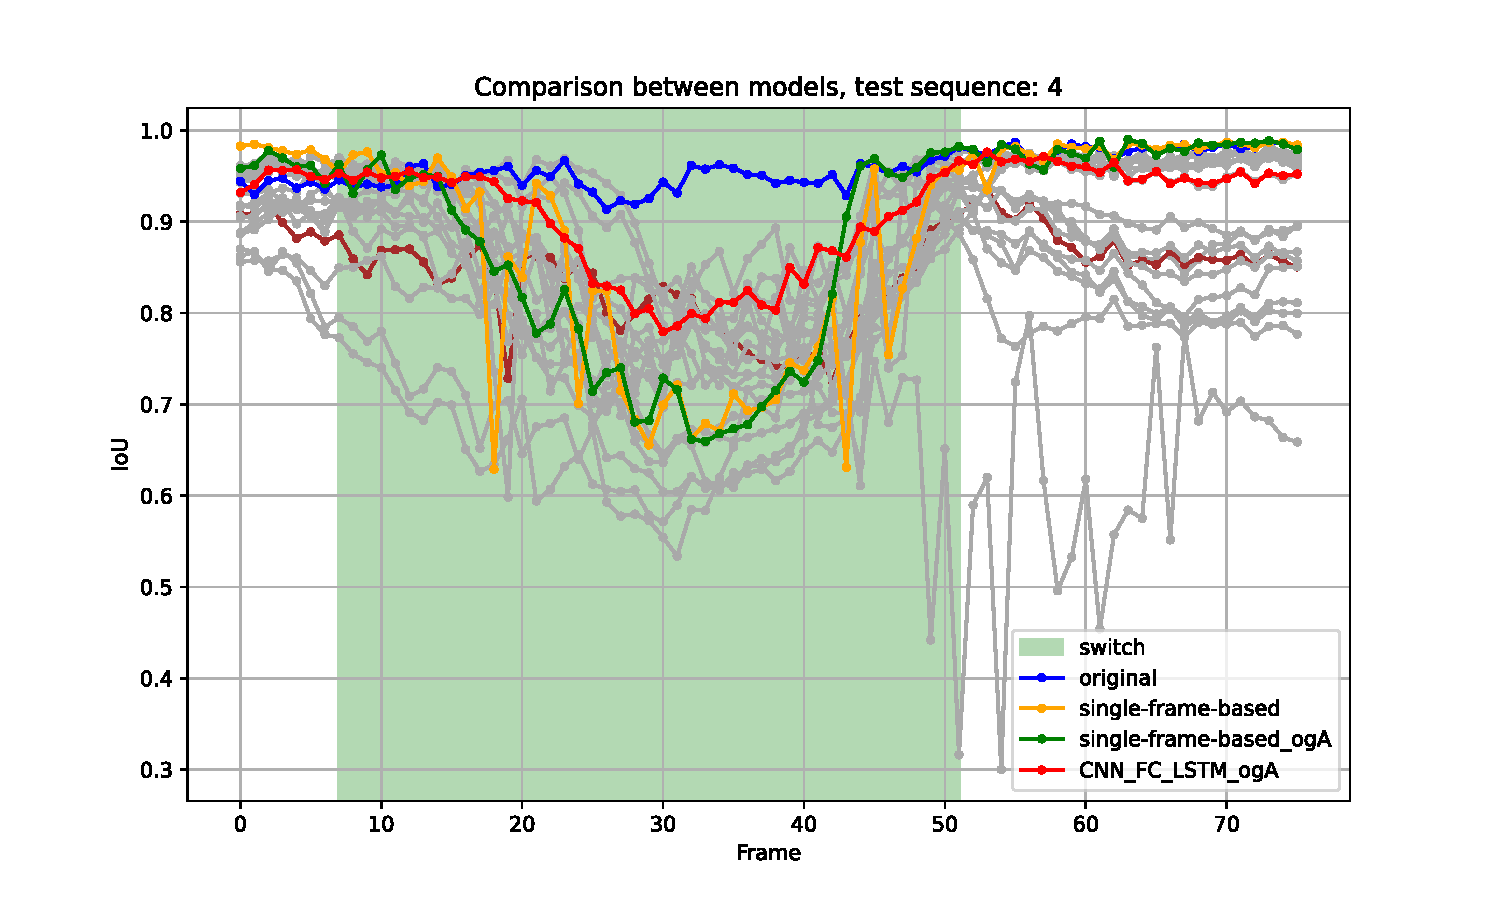
\includegraphics[width=\textwidth]{PICs/experiments/temporalModels/plot_ious_sequence_4.pdf}
        \caption{\textbf{Switch 1} (single-frame model: 76/76 frames correct)}
        \label{fig:IoUTrends_switch_4}
    \end{subfigure}
    \begin{subfigure}[b]{0.49\textwidth}
        \centering
        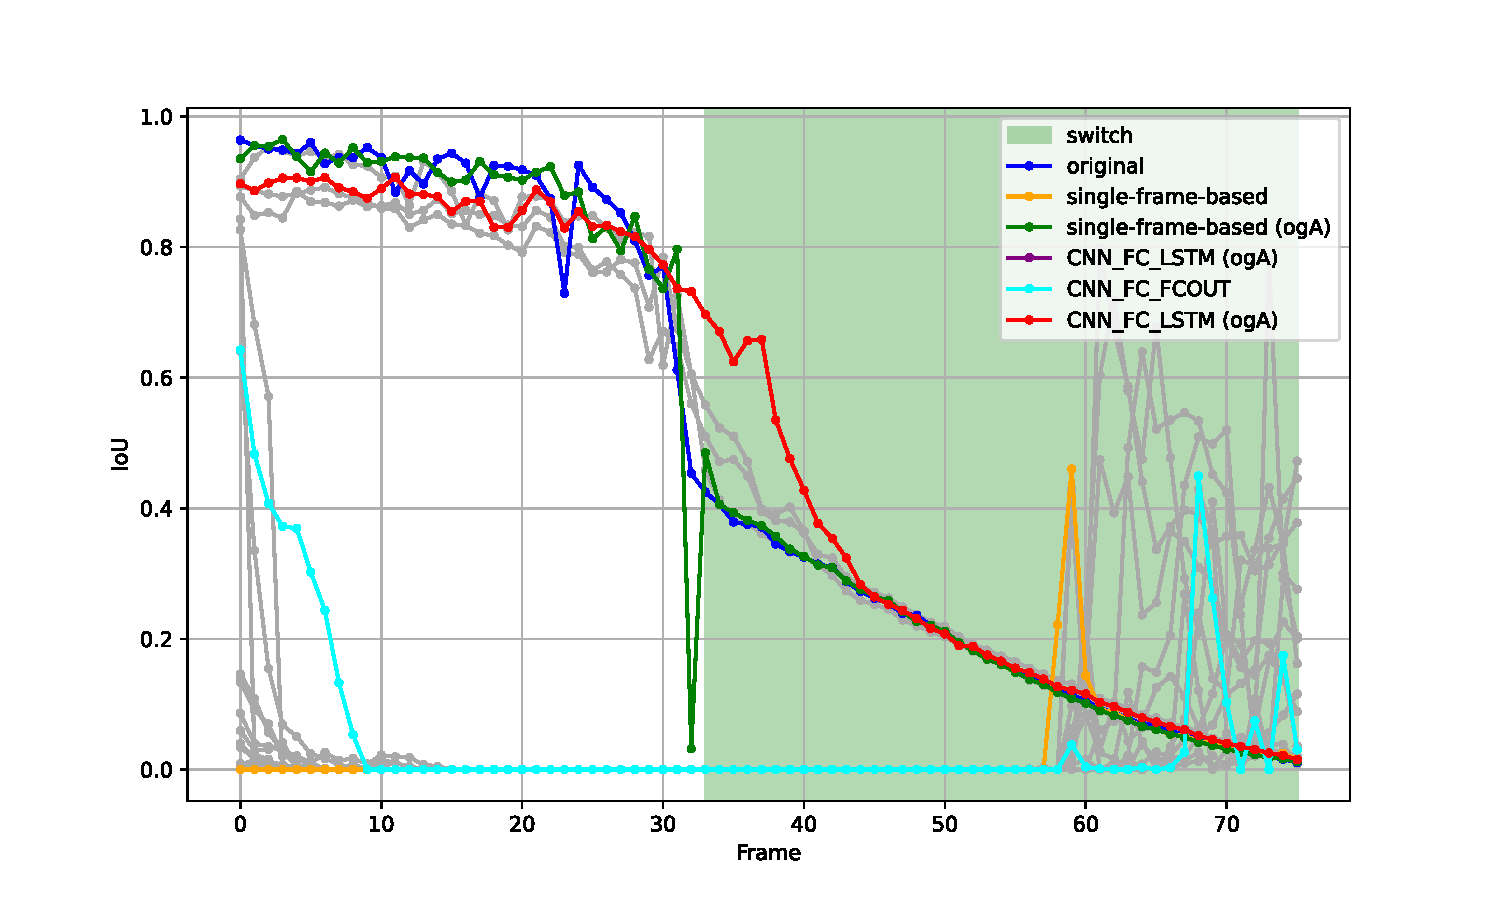
\includegraphics[width=\textwidth]{PICs/experiments/temporalModels/plot_ious_sequence_2.pdf}
        \caption{\textbf{Switch 2} (single-frame model: 0/76 frames correct)}
        \label{fig:IoUTrends_switch_2}
    \end{subfigure}

    \vspace{0.2em} % Kleiner vertikaler Abstand

    \begin{subfigure}[b]{0.49\textwidth}
        \centering
        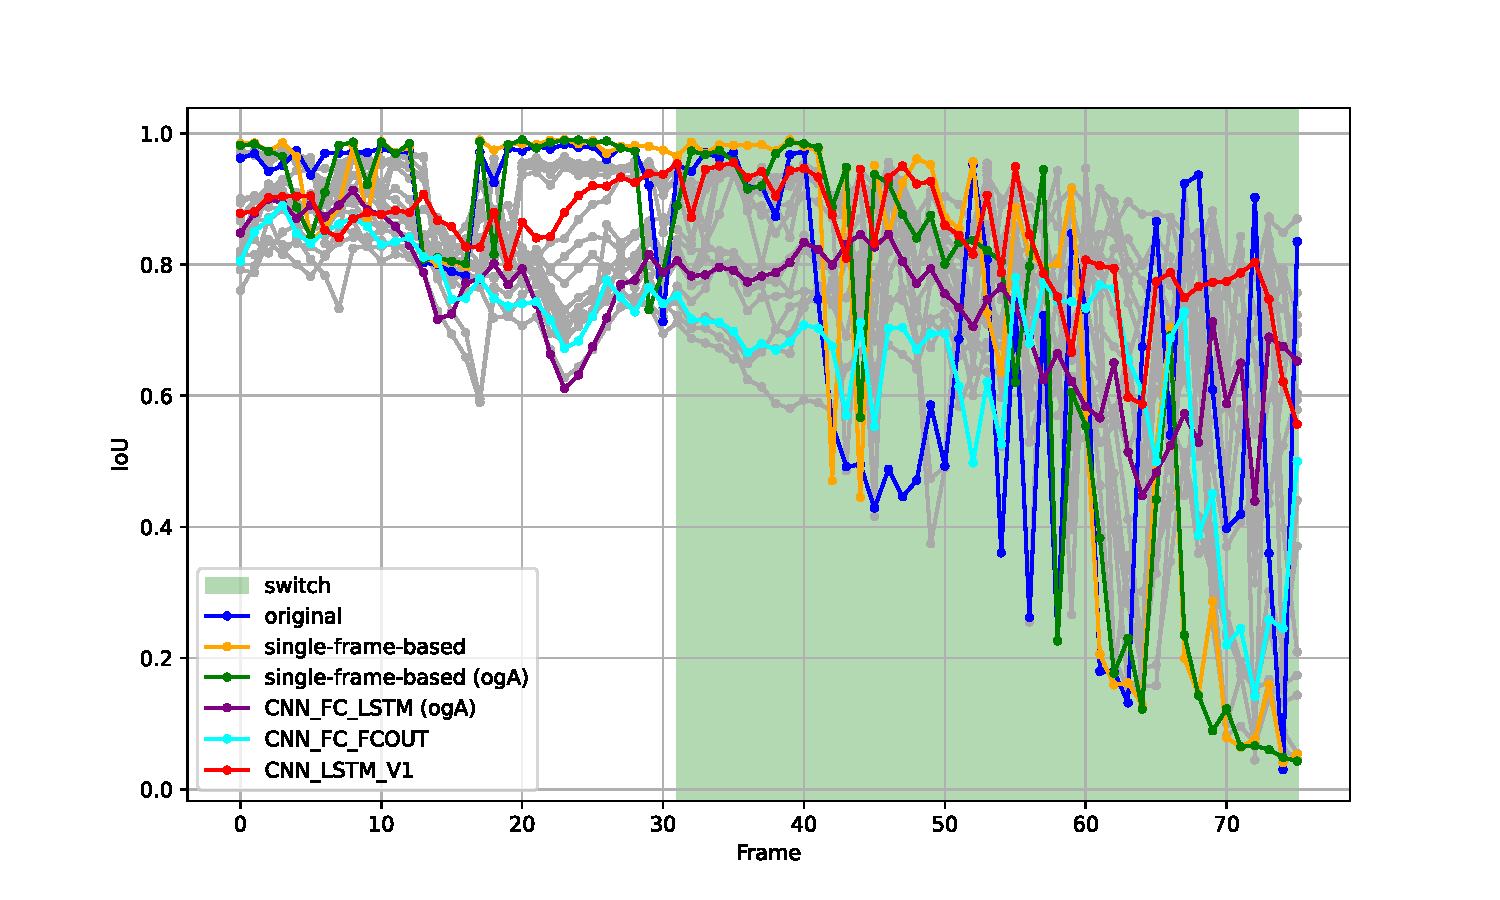
\includegraphics[width=\textwidth]{PICs/experiments/temporalModels/plot_ious_sequence_3.pdf}
        \caption{\textbf{Switch 3} (single-frame model: 36/76 frames correct)}
        \label{fig:IoUTrends_switch_3}
    \end{subfigure}
    \begin{subfigure}[b]{0.49\textwidth}
        \centering
        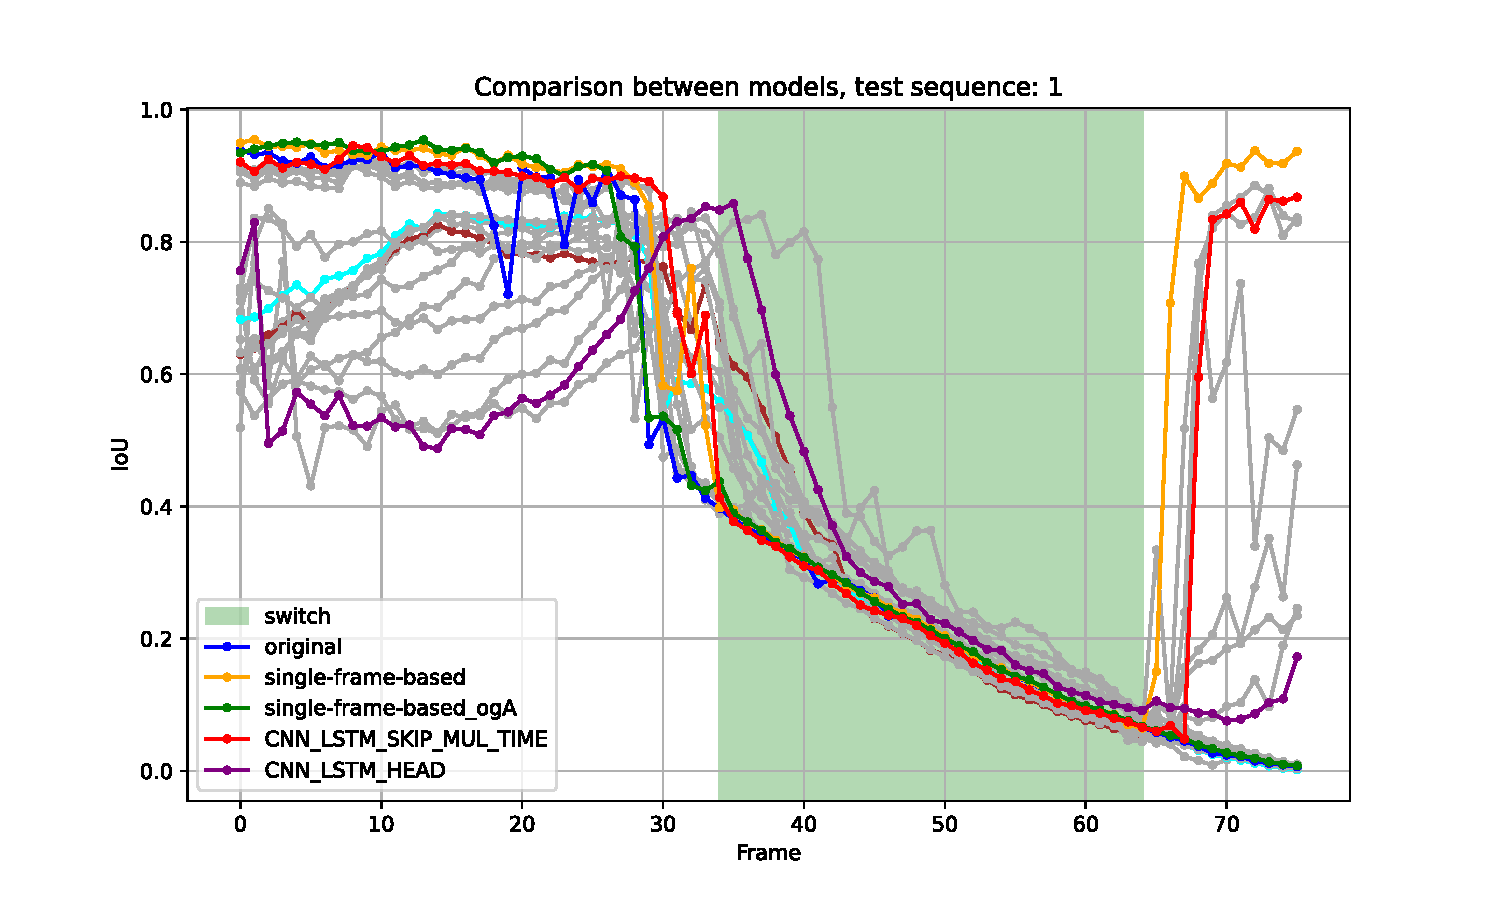
\includegraphics[width=\textwidth]{PICs/experiments/temporalModels/plot_ious_sequence_1.pdf}
        \caption{\textbf{Switch 4} (single-frame model: 39/76 frames correct)}
        \label{fig:IoUTrends_switch_1}
    \end{subfigure}

    \caption{\ac{IoU}-Trends of all models on the temporal test dataset with four sequences. Red is the best-performing temporal model for the corresponding sequence.}
    \label{fig:IoUTrends}
\end{figure}

%\begin{figure}[H]
%    \centering
%    \begin{subfigure}[t]{0.8\textwidth}
%        \centering
%        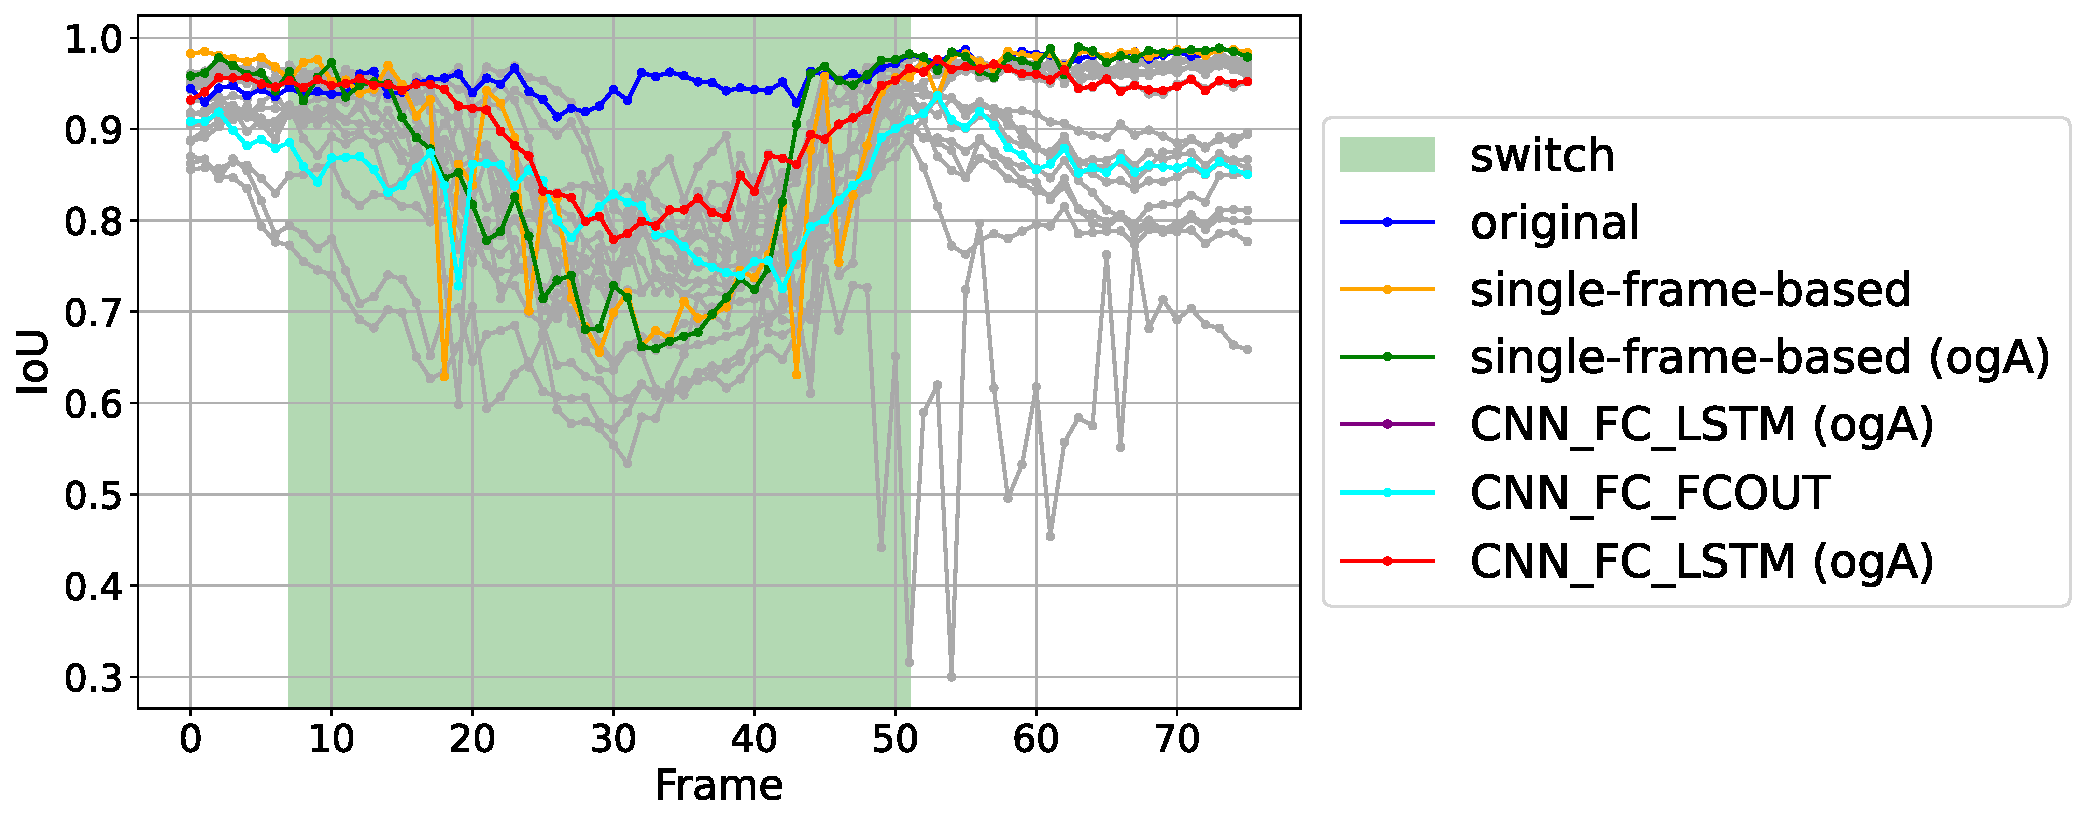
\includegraphics[width=\textwidth]{PICs/experiments/temporalModels/plot_ious_sequence_4_updated_v2.pdf}
%        \caption{\textbf{Switch 1} (single-frame model: 76/76 frames correct)}
%        \label{fig:IoUTrends_switch_4}
%    \end{subfigure}
%
%    %\vspace{1em} % Größerer vertikaler Abstand
%
%    \begin{subfigure}[t]{0.8\textwidth}
%        \centering
%        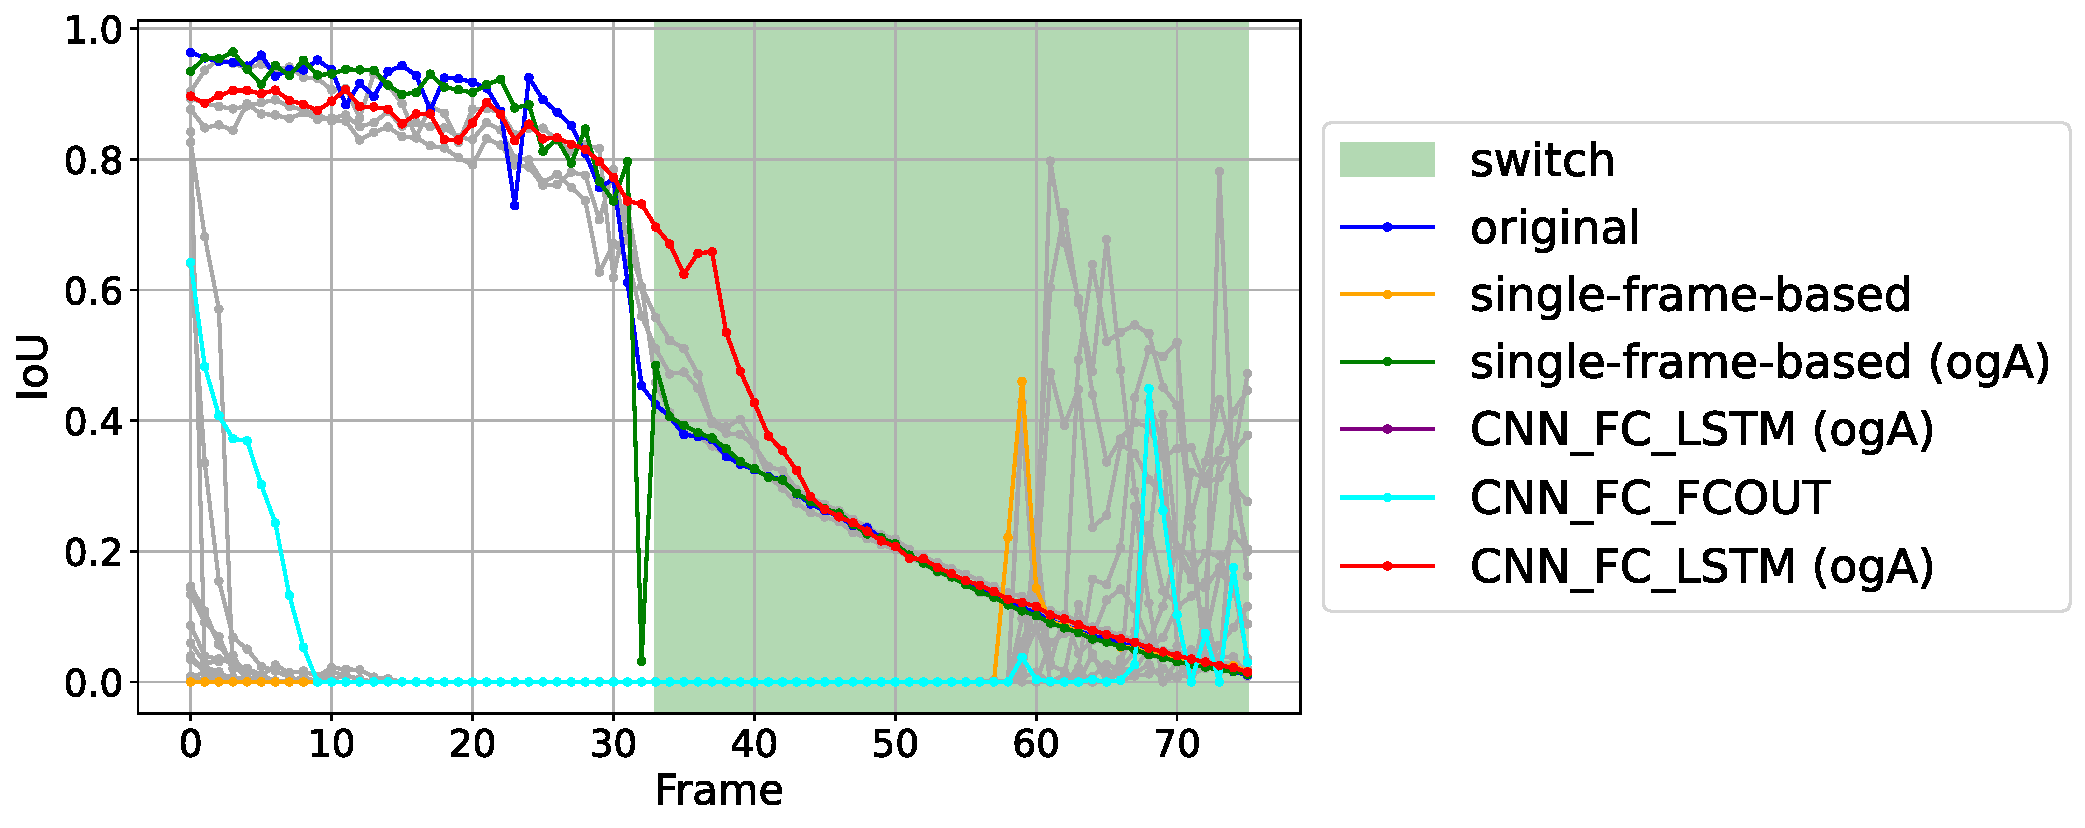
\includegraphics[width=\textwidth]{PICs/experiments/temporalModels/plot_ious_sequence_2_updated_v2.pdf}
%        \caption{\textbf{Switch 2} (single-frame model: 0/76 frames correct)}
%        \label{fig:IoUTrends_switch_2}
%    \end{subfigure}
%
%    %\vspace{1em} % Größerer vertikaler Abstand
%
%    \begin{subfigure}[t]{0.8\textwidth}
%        \centering
%        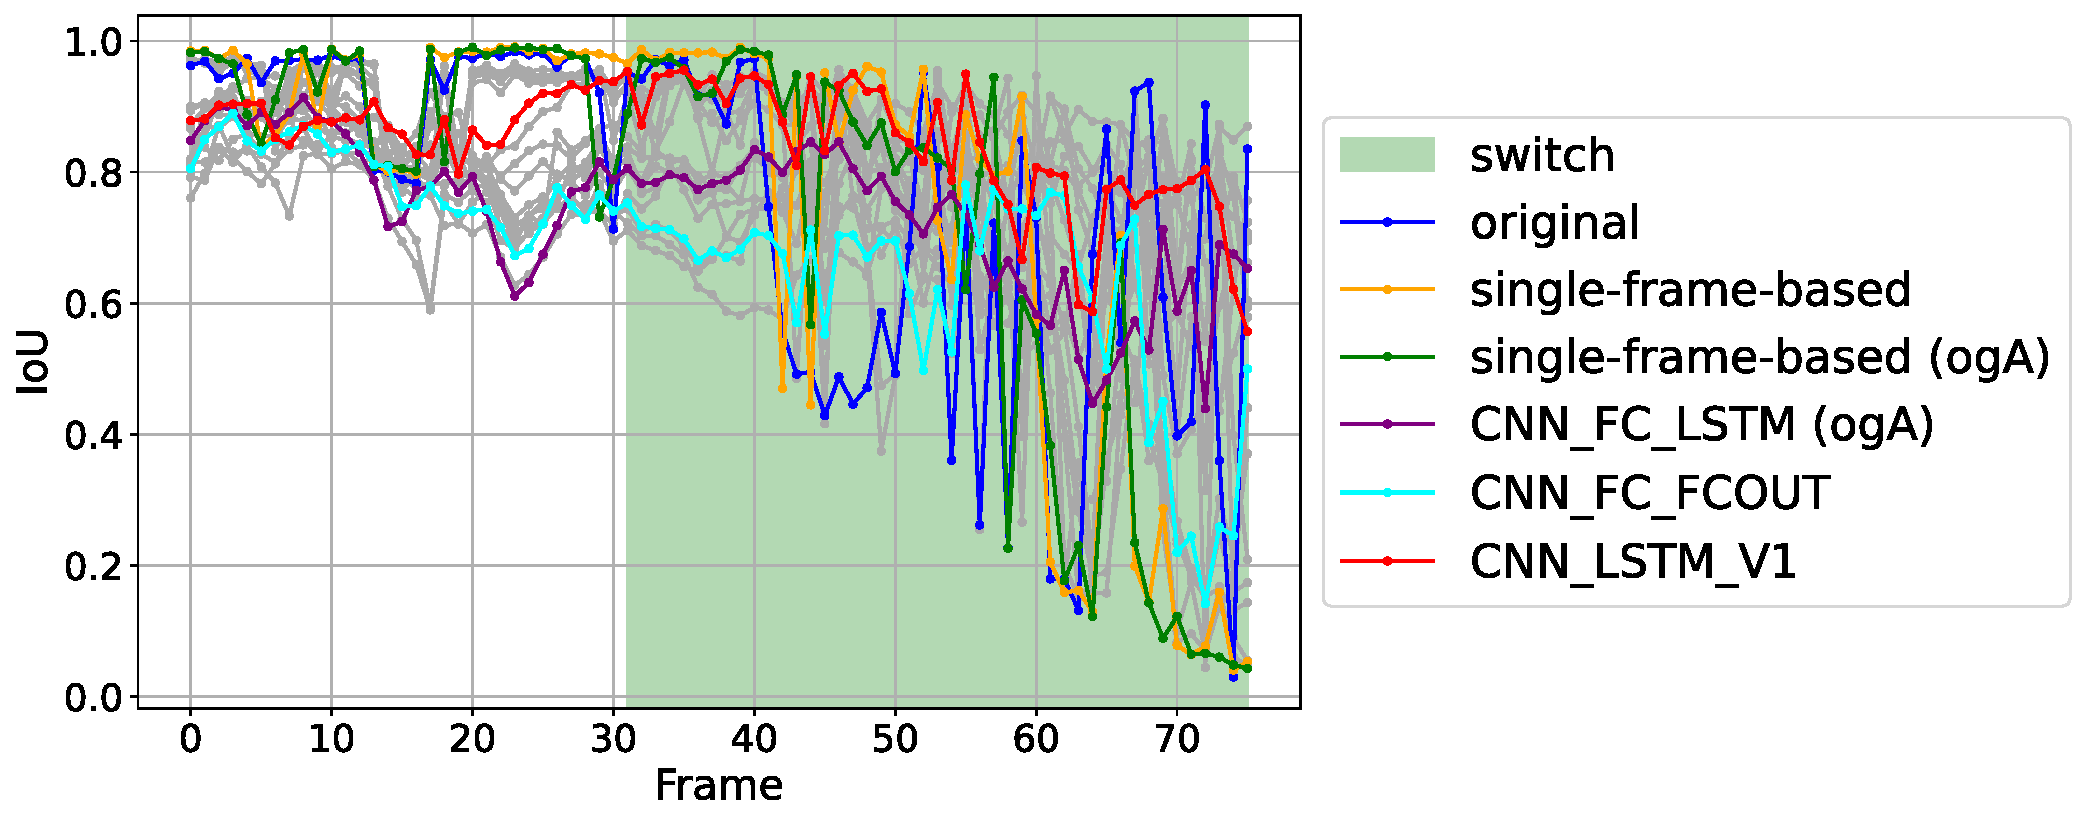
\includegraphics[width=\textwidth]{PICs/experiments/temporalModels/plot_ious_sequence_3_updated_v2.pdf}
%        \caption{\textbf{Switch 3} (single-frame model: 36/76 frames correct)}
%        \label{fig:IoUTrends_switch_3}
%    \end{subfigure}
%
%    %\vspace{1em} % Größerer vertikaler Abstand
%
%    \begin{subfigure}[t]{0.8\textwidth}
%        \centering
%        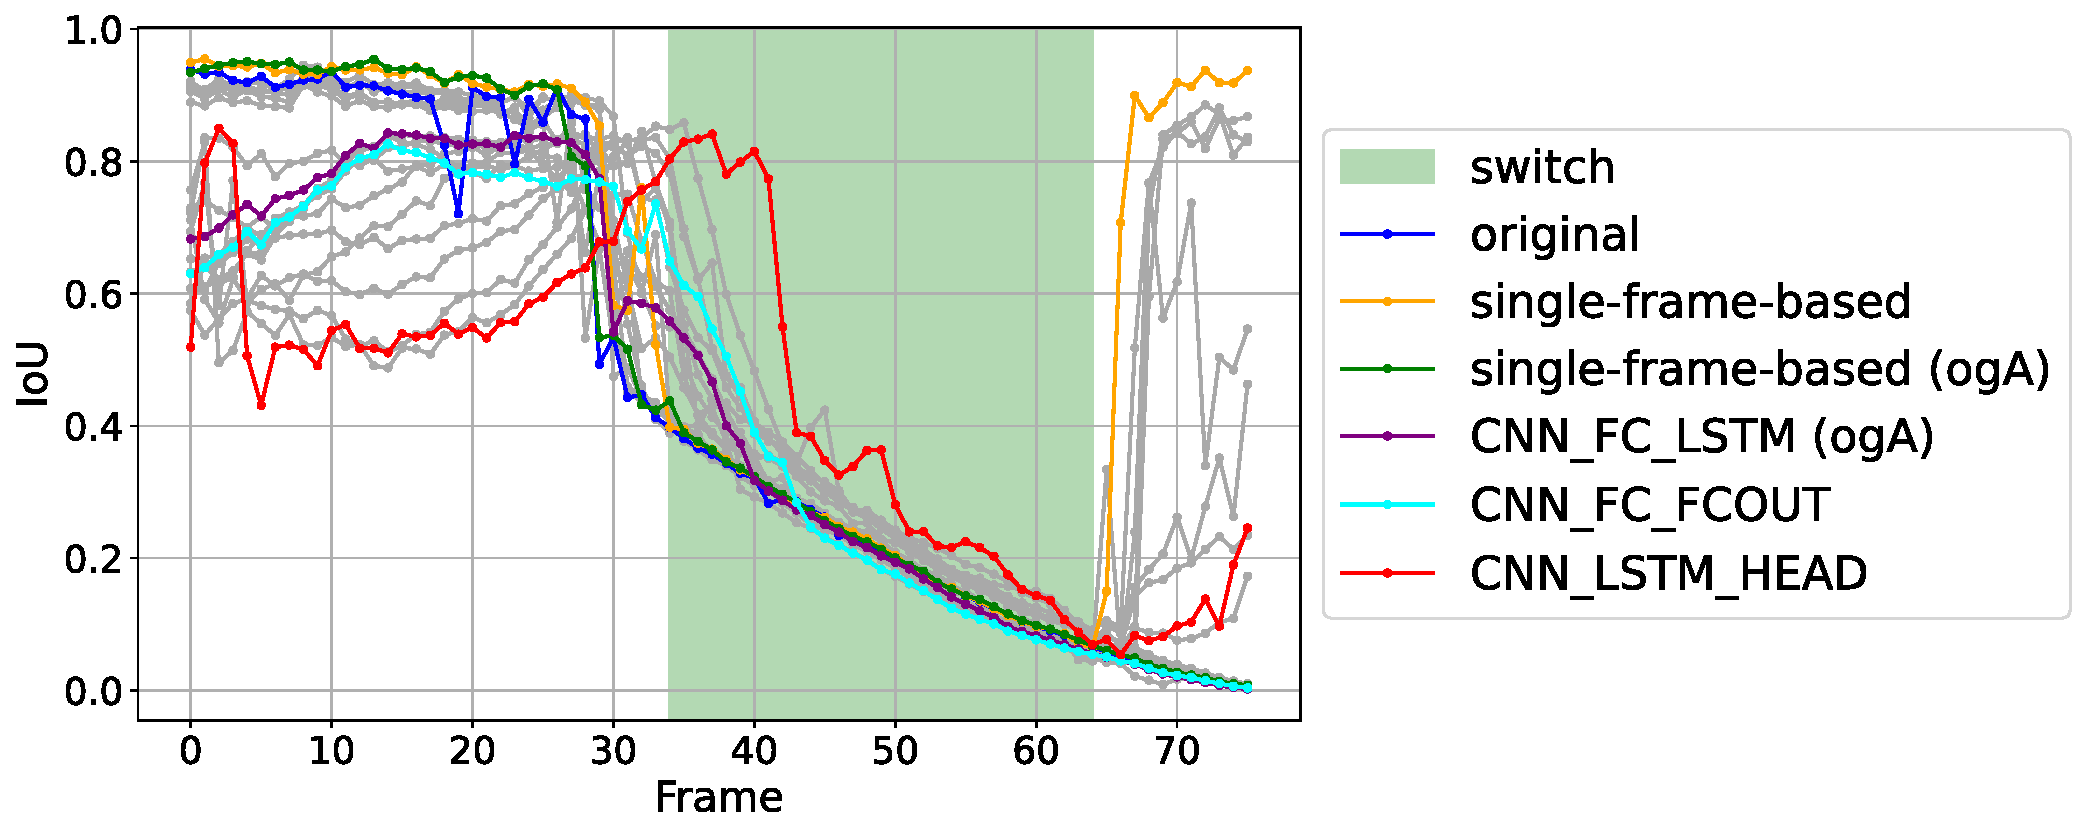
\includegraphics[width=\textwidth]{PICs/experiments/temporalModels/plot_ious_sequence_1_updated_v2.pdf}
%        \caption{\textbf{Switch 4} (single-frame model: 39/76 frames correct)}
%        \label{fig:IoUTrends_switch_1}
%    \end{subfigure}
%
%    \caption{\ac{IoU}-Trends of all models on the temporal test dataset with four sequences. Red is the best-performing temporal model for the corresponding sequence.}
%    \label{fig:IoUTrends}
%\end{figure}


\begin{table}[H]
    \centering
    \resizebox{\textwidth}{!}{
    \begin{tabular}{lcccc}
        \hline
        \rowcolor{white} \textbf{} & \textbf{Switch 1} & \textbf{Switch 2} & \textbf{Switch 3} & \textbf{Switch 4} \\
        \hline
        \rowcolor[gray]{0.9} TEP Net \cite{tepNet2024} IoU & 94.76 \%            & 18.47 \%          & 63.96 \%              & 22.10 \%        \\
        \rowcolor{white}     single-frame-based IoU        & 81.99 \%            &  3.68 \%          & 65.99 \%              & 22.43 \%        \\
        \rowcolor[gray]{0.9} single-frame-based (ogA) IoU  & 82.74 \%            & 18.56 \%          & 63.85 \%              & 22.57 \%        \\
        \rowcolor{white}     best temporal model           & CNN\_FC\_LSTM (ogA) & CNN\_FC\_LSTM (ogA) & CNN\_LSTM\_V1   & CNN\_LSTM\_HEAD \\
        \rowcolor[gray]{0.9} best temporal model IoU       & 88.23 \%            & 23.43 \%          & 83.77 \%              & 40.59 \%        \\
        \hline
    \end{tabular}
    }
    \caption{Temporal Models Results Switches}
    \label{tab:temporalModelsResultsIoUsSummary}
\end{table}

\autoref{tab:temporalModelsResults} presents a thorough evaluation.
Each model is evaluated on the four test sequences, and an average of all switch \ac{IoU}s is given.
Additionally, an average of only the first and the third switch is included in \autoref{tab:temporalModelsResults}.
The reason for that lies in the particular scenarios of \textbf{Switch 1} and \textbf{Switch 2}.
\autoref{fig:temporalTestSet} shows the first frame of each sequence and the number of frames that are predicted correctly from the single-frame-based model.
In the video of \textbf{Switch 2}, 0/76 frames are predicted, which shows the complexity of this particular scene.
In \textbf{Switch 1}, all frames are correctly predicted, which shows that the single-frame-based model has no issues predicting this scene.
In general, there are switches where the track splits.
However, only one route diverges, and the rail on which the train continues remains on a straight path.
The \textbf{Switch 1} sequence is such a scenario therefore it is similar to a rail without any switches.
The reason the original model performed with such high accuracy lies mainly in the original auto-crop mechanism.
This method uses an \ac{RA}, so the crop coordinates coverage to global averages.
This characteristic presents a disadvantage in most cases because it cannot adapt to different scenarios.
However, in the cases of \textbf{Switch 1} and \textbf{Switch 2}, the behavior of not adapting to a new situation presents an advantage.
Therefore, especially in those two scenes, the utilization of the original auto-crop is advantageous.
It must be mentioned that the high accuracy is highly dependent on these two particular situations.
This work focuses more on scenarios in which models correctly predict the track before the train drives over a switch, and only when the starting context of the switch is missing should the temporal model achieve an improvement.
This situation occurs in scenarios \textbf{Switch 3} and \textbf{Switch 4}.
Therefore, the additional average of just these two scenes is included in \autoref{tab:temporalModelsResults}.

\autoref{tab:temporalModelsResults} shows that even when scenarios \textbf{Switch 1} and \textbf{Switch 2} are included, a temporal model (CNN\_FC\_LSTM (ogA)) still achieves the highest overall accuracy.
When excluding those two scenes as expected, a temporal model with the adapted auto-crop mechanism (CNN\_FC\_FCOUT\_V1) outperforms other techniques.

\begin{table}[H]
    \centering
    \resizebox{\textwidth}{!}{
    \begin{tabular}{lccccccc}
        \hline
        \rowcolor{white} \textbf{Model} & \textbf{original Autocrop} & \textbf{Switch 1} & \textbf{Switch 2} & \textbf{Switch 3} & \textbf{Switch 4} & \textbf{AVG all Switches} & \textbf{AVG Switch 3 \& 4} \\
        \hline
        \rowcolor[gray]{0.9} TEP Net \cite{tepNet2024}    & \checkmark & \textbf{94.76 \%} & 18.47 \%          & 63.96 \%          & 22.10 \%          & 49.82 \%          & 43.03 \%          \\ 
        \rowcolor{white}     single-frame-based           &            & 81.99 \%          &  3.68 \%          & 65.99 \%          & 22.43 \%          & 43.53 \%          & 44.21 \%          \\ 
        \rowcolor[gray]{0.9} single-frame-based           & \checkmark & 82.74 \%          & 18.56 \%          & 63.85 \%          & 22.57 \%          & 46.93 \%          & 43.21 \%          \\ 
        \hline
        \rowcolor[gray]{0.9} CNN\_FC\_LSTM                &            & 84.47 \%          &  6.77 \%          & 70.01 \%          & 23.89 \%          & 46.29 \%          & 46.95 \%          \\ 
        \rowcolor{white}     CNN\_LSTM\_V1                &            & 69.55 \%          &  4.70 \%          & \textbf{83.77 \%} & 26.40 \%          & 46.10 \%          & 55.09 \%          \\ 
        \rowcolor[gray]{0.9} CNN\_LSTM\_V2                &            & 79.15 \%          &  0.64 \%          & 78.86 \%          & 32.11 \%          & 42.79 \%          & 43.30 \%          \\ 
        \rowcolor{white}     CNN\_LSTM\_HEAD              &            & 78.33 \%          &  3.05 \%          & 78.32 \%          & \textbf{40.59 \%} & 47.69 \%          & 55.49 \%          \\ 
        \rowcolor[gray]{0.9} CNN\_FC\_FCOUT\_V1           &            & 81.86 \%          &  2.71 \%          & 61.49 \%          & 25.11 \%          & 50.07 \%          & \textbf{59.46 \%} \\ 
        \rowcolor{white}     CNN\_FC\_FCOUT\_V2           &            & 86.68 \%          &  3.76 \%          & 61.82 \%          & 23.59 \%          & 47.76 \%          & 56.18 \%          \\ 
        \rowcolor[gray]{0.9} CNN\_FLAT\_FC                &            & 78.24 \%          &  0.46 \%          & 81.88 \%          & 30.47 \%          & 43.96 \%          & 42.70 \%          \\ 
        \rowcolor{white}     CNN\_LSTM\_SKIP\_CAT         &            & 82.83 \%          &  2.08 \%          & 70.02 \%          & 22.58 \%          & 44.38 \%          & 46.30 \%          \\ 
        \rowcolor[gray]{0.9} CNN\_LSTM\_SKIP\_MUL\_FRAME  &            & 84.38 \%          &  3.18 \%          & 72.55 \%          & 22.29 \%          & 45.60 \%          & 47.42 \%          \\ 
        \rowcolor{white}     CNN\_LSTM\_SKIP\_MUL\_TIME   &            & 83.96 \%          &  5.52 \%          & 65.90 \%          & 21.49 \%          & 44.22 \%          & 43.69 \%          \\ 
        \hline
        \rowcolor[gray]{0.9} CNN\_FC\_LSTM                & \checkmark & 88.23 \%          & \textbf{23.43 \%} & 70.35 \%          & 23.65 \%          & \textbf{51.41 \%} & 47.00 \%          \\ 
        \rowcolor{white}     CNN\_LSTM\_V1                & \checkmark & 72.51 \%          & 14.82 \%          & 80.69 \%          & 26.22 \%          & 48.56 \%          & 53.46 \%          \\ 
        \rowcolor[gray]{0.9} CNN\_LSTM\_V2                & \checkmark & 75.99 \%          & 13.44 \%          & 76.83 \%          & 28.50 \%          & 45.72 \%          & 39.42 \%          \\ 
        \rowcolor{white}     CNN\_LSTM\_HEAD              & \checkmark & 76.68 \%          &  9.93 \%          & 80.15 \%          & 30.61 \%          & 48.69 \%          & 52.66 \%          \\ 
        \rowcolor[gray]{0.9} CNN\_FC\_FCOUT\_V1           & \checkmark & 83.60 \%          & 20.43 \%          & 55.45 \%          & 23.40 \%          & 49.34 \%          & 55.38 \%          \\ 
        \rowcolor{white}     CNN\_FC\_FCOUT\_V2           & \checkmark & 85.92 \%          & 20.07 \%          & 59.29 \%          & 21.40 \%          & 50.60 \%          & 54.25 \%          \\ 
        \rowcolor[gray]{0.9} CNN\_FLAT\_FC                & \checkmark & 80.54 \%          & 13.35 \%          & 80.70 \%          & 27.80 \%          & 46.67 \%          & 40.35 \%          \\ 
        \rowcolor{white}     CNN\_LSTM\_SKIP\_CAT         & \checkmark & 85.37 \%          &  4.43 \%          & 78.36 \%          & 22.92 \%          & 47.77 \%          & 50.64 \%          \\ 
        \rowcolor[gray]{0.9} CNN\_LSTM\_SKIP\_MUL\_FRAME  & \checkmark & 86.57 \%          &  2.27 \%          & 77.05 \%          & 22.85 \%          & 47.18 \%          & 49.95 \%          \\ 
        \rowcolor{white}     CNN\_LSTM\_SKIP\_MUL\_TIME   & \checkmark & 85.35 \%          & 18.34 \%          & 64.79 \%          & 22.53 \%          & 47.75 \%          & 43.66 \%          \\ 
        \hline
    \end{tabular}
    }
    \caption{Temporal Models Results IoUs}
    \label{tab:temporalModelsResults}
\end{table}

%\begin{table}[H]
%    \centering
%    \resizebox{\textwidth}{!}{
%    \begin{tabular}{lcccccccccc}
%        \hline
%        \rowcolor{white} \textbf{Model} & \textbf{Testset} & \textbf{Sequence 1} & \textbf{Sequence 2} & \textbf{Sequence 3} & \textbf{Sequence 4} & \textbf{Switch 1} & \textbf{Switch 2} & \textbf{Switch 3} & \textbf{Switch 4} & \textbf{switch averages} \\
%        \hline
%        \rowcolor[gray]{0.9} single-frame-based           & 57.03 \%          & 60.66 \%          & 2.06 \%                            & 76.75 \%                            & 88.66 \%                            & 22.43 \%                            & 3.60 \%                            & 65.99 \%                            & 81.99 \%                            & 43.5 \%\\ 
%        \hline
%        \rowcolor{white}     CNN\_LSTM\_FC                & \multicolumn{10}{c}{canceled at epoch 107: no generalization} \\ 
%        \rowcolor[gray]{0.9} CNN\_FC\_LSTM                & 52.88 \%          & 43.60 \%          & \textcolor{blue}{4.22 \%}          & 74.71 \%                            & \textcolor{blue}{88.99 \%}          & \textcolor{blue}{23.89 \%}          & \textcolor{blue}{\textbf{6.61 \%}} & \textcolor{blue}{70.01 \%}          & \textcolor{blue}{84.47} \%          & 46.25 \% \\ 
%        \rowcolor{white}     CNN\_LSTM\_V1                & 52.93 \%          & 45.80 \%          & \textcolor{blue}{3.42 \%}          & \textcolor{blue}{85.19 \%}          & 77.29 \%                            & \textcolor{blue}{26.40 \%}          & \textcolor{blue}{4.59 \%}          & \textcolor{blue}{\textbf{83.77 \%}} & 69.55 \%                            & 46.08 \% \\ 
%        \rowcolor[gray]{0.9} CNN\_LSTM\_V2                & 50.96 \%          & 41.50 \%          & 0.76 \%                            & \textcolor{blue}{80.08 \%}          & 81.49 \%                            & \textcolor{blue}{32.11 \%}          & 0.62 \%                            & \textcolor{blue}{78.86 \%}          & 79.15 \%                            & 42.78 \% \\ 
%        \rowcolor{white}     CNN\_LSTM\_HEAD              & 52.04 \%          & 44.34 \%          & \textcolor{blue}{2.19 \%}          & \textcolor{blue}{80.19 \%}          & 81.44 \%                            & \textcolor{blue}{\textbf{40.59 \%}} & 2.98 \%                            & \textcolor{blue}{78.32 \%}          & 78.33 \%                            & 47.69 \% \\ 
%        \rowcolor[gray]{0.9} CNN\_FC\_FCOUT\_V1           & 50.57 \%          & 43.88 \%          & \textcolor{blue}{\textbf{5.49 \%}} & 68.44 \%                            & 84.47 \%                            & \textcolor{blue}{25.11 \%}          & 2.65 \%                            & 61.49 \%                            & 81.86 \%                            & 50.05 \% \\ 
%        \rowcolor{white}     CNN\_FC\_FCOUT\_V2           & 53.35 \%          & 50.59 \%          & \textcolor{blue}{4.05 \%}          & 68.22 \%                            & \textcolor{blue}{\textbf{90.52 \%}} & \textcolor{blue}{23.59 \%}          & \textcolor{blue}{3.67 \%}          & 61.82 \%                            & \textcolor{blue}{\textbf{86.68 \%}} & 47.76 \% \\ 
%        \rowcolor[gray]{0.9} CNN\_FLAT\_FC                & 50.17 \%          & 42.81 \%          & 0.75 \%                            & \textcolor{blue}{83.01 \%}          & 74.08 \%                            & \textcolor{blue}{30.47 \%}          & 0.45 \%                            & \textcolor{blue}{81.88 \%}          & 78.24 \%                            & 43.94 \% \\ 
%        \rowcolor{white}     CNN\_LSTM\_SKIP\_CAT         & 56.17 \%          & 56.27 \%          & 1.17 \%                            & \textcolor{blue}{78.66 \%}          & 88.58 \%                            & \textcolor{blue}{22.58 \%}          & 2.03 \%                            & \textcolor{blue}{70.02 \%}          & \textcolor{blue}{82.83 \%}          & 44.37 \% \\ 
%        \rowcolor[gray]{0.9} CNN\_LSTM\_SKIP\_MUL\_FRAME  & \textbf{56.97 \%} & 56.31 \%          & 1.79 \%                            & \textcolor{blue}{\textbf{80.27 \%}} & \textcolor{blue}{89.51 \%}          & 22.29 \%                            & 3.11 \%                            & \textcolor{blue}{72.55 \%}          & \textcolor{blue}{84.38 \%}          & 45.58 \% \\ 
%        \rowcolor{white}     CNN\_LSTM\_SKIP\_MUL\_TIME   & 56.41 \%          & \textbf{57.12 \%} & \textcolor{blue}{3.41 \%}          & 75.68 \%  	                         & \textcolor{blue}{89.45 \%}          & \textcolor{blue}{21.49 \%}          & \textcolor{blue}{5.39 \%}          & 65.90 \%                            & \textcolor{blue}{83.96 \%}          & 44.18 \% \\ 
%        \hline
%        \rowcolor[gray]{0.9} best with MNV3-Small & xy \% & xy \% & xy \% & xy \% & xy \% & xy \% & xy \% & xy \% & xy \% & xy \% \\
%        \rowcolor{white}     best with MNV3-Large & xy \% & xy \% & xy \% & xy \% & xy \% & xy \% & xy \% & xy \% & xy \% & xy \% \\
%        \hline
%    \end{tabular}
%    }
%    \caption{Temporal Models Results IoUs}
%    \label{tab:temporalModelsResultsIoUs_old}
%\end{table}

\begin{table}[H]
    \centering
    \resizebox{\textwidth}{!}{
    \begin{tabular}{lcccc}
        \hline
        \rowcolor{white} \textbf{Model} & \textbf{Parameters} & \textbf{Flops} & \textbf{MACs} & \textbf{Latency TRT FP32 / FP16} \\
        \hline
        \rowcolor[gray]{0.9} single-frame-based          & 32.92M & 10.17B & 5.38G & 25.87 / 16.09 ms \\ 
        \hline
        \rowcolor{white}     CNN\_LSTM\_FC               & \multicolumn{4}{c}{canceled at epoch 107: no generalization} \\ 
        \rowcolor[gray]{0.9} CNN\_FC\_LSTM               & 32.87M  & 101.72B & 53.81G & \textbf{223.07} / 129.69 ms \\ 
        \rowcolor{white}     CNN\_LSTM\_V1               & \textbf{11.10M}  & \textbf{101.28B} & \textbf{53.59G} & 246.90 / 156.04 ms \\ 
        \rowcolor[gray]{0.9} CNN\_LSTM\_V2               & 13.62M  & 101.33B & 53.62G & 246.94 / 155.09 ms \\ 
        \rowcolor{white}     CNN\_LSTM\_HEAD             & 13.15M  & 101.32B & 53.61G & 247.11 / 136.35 ms \\ 
        \rowcolor[gray]{0.9} CNN\_FC\_FCOUT\_V1          & 33.08M  & 101.72B & 53.81G & 265.14 / 128.91 ms \\ 
        \rowcolor{white}     CNN\_FC\_FCOUT\_V2          & 35.50M  & 101.72B & 53.81G & 328.86 / 156.09 ms \\ 
        \rowcolor[gray]{0.9} CNN\_FLAT\_FC               & 132.21M & 101.52B & 53.71G & 230.06 / \textbf{127.88} ms \\ 
        \rowcolor{white}     CNN\_LSTM\_SKIP\_CAT        & 35.05M  & 101.36B & 53.63G & 223.87 / 131.76 ms \\ 
        \rowcolor[gray]{0.9} CNN\_LSTM\_SKIP\_MUL\_FRAME & 35.04M  & 101.76B & 53.83G & 227.75 / 130.14 ms \\ 
        \rowcolor{white}     CNN\_LSTM\_SKIP\_MUL\_TIME  & 35.05M  & 101.76B & 53.83G & 265.56 / 130.15 ms \\ 
        \hline
        \rowcolor[gray]{0.9} CNN\_FLAT\_FC with MNV3-Small & 122.48M & 6.66B & 3.64G & 25.41 / 15.02 ms \\
        \hline
    \end{tabular}
    }
    \caption{Temporal Models Results}
    \label{tab:temporalModelsResultsLatency}
\end{table}


\autoref{tab:temporalModelsResultsLatency} shows the results for temporal Models considering Parameters, Flops, MACs, and the Latency measured on the NVIDIA Jetson device.
Compared to the single-frame-based model, temporal ones are slower, with FP16 latencies between 127.88 ms and 156.09 ms and FP32 latencies between 223.07 ms and 328.86 ms.
The fastest model is the CNN\_FLAT\_FC on FP16 with 127.88 ms, corresponding to a frame rate of 7.8 \ac{FPS}.
When inferring videos with 30 \ac{FPS}, these models are not real-time capable anymore.
However, there are methods to enable real-time capability for these temporal models.
For example switching the backbone to a MobileNet-Small, as given in \autoref{tab:temporalModelsResultsLatency}.
This significantly reduces latency and falls below the real-time threshold of 33.33 ms.
Nevertheless, this topic falls outside the scope of this work and is therefore addressed in \autoref{sec:discussion}.
In this study, no temporal models utilizing a MobileNet backbone have been examined concerning their accuracy.
Only the latency is measured.